\section{The benchmark: a 12-site kagome Heisenberg star}
\label{sec:problem}

The variational quantum eigensolver (VQE) \parencite{peruzzo2014} prepares a parameterised
state $\ket{\psi(\theta)}$ on a quantum device, measures its energy, and lets a classical
optimiser lower that energy. The 2022 IBM Open Science Prize \parencite{ibmprize2022} asked for
the ground-state energy of a small kagome antiferromagnet to within $1\,\%$ relative error on
\texttt{ibmq\_guadalupe}. This section fixes the model and proves what its ground state is.
Everything later depends on that answer.

\subsection{Lattice and Hamiltonian}

\begin{dfn}[Kagome star]\label{dfn:star}
  The \emph{kagome star} is the graph $\Lambda=(V,E)$ with sites $V=\{0,\dots,11\}$ and
  \VNumBonds{} bonds
  \[
    E=\underbrace{\bigl\{\{i,i+1\}\bigr\}_{i=0}^{5}}_{\text{hexagon}}\;\cup\;
    \underbrace{\bigl\{\{i,6+i\},\ \{i+1,6+i\}\bigr\}_{i=0}^{5}}_{\text{spokes}},
  \]
  with indices of hexagon sites taken modulo $6$. Sites $0$--$5$ form a hexagon; tip $6+i$
  caps the hexagon edge $\{i,i+1\}$ and closes the triangle
  \[
    \tau_i=\{i,\ i+1,\ 6+i\},\qquad i=0,\dots,5 .
  \]
\end{dfn}

The six triangles share corners but no bonds: each of the \VNumBonds{} bonds lies in exactly one
triangle, because $\tau_i$ contains the hexagon bond $\{i,i+1\}$ and the two spokes of tip
$6+i$, and nothing else. This partition is the key to the whole analysis.
Hexagon sites have degree $4$ and tips degree $2$. The package stores this graph as
\py{kagome_vqe.lattice.KAGOME_UNIT_CELL_EDGES}; Figure~\ref{fig:lattice}(a) draws it.

\begin{dfn}[Heisenberg Hamiltonian]\label{dfn:ham}
  On $(\CC^2)^{\otimes 12}$, with Pauli operators $X_i,Y_i,Z_i$ on site $i$,
  \[
    H=\sum_{\{i,j\}\in E} h_{ij},\qquad h_{ij}=X_iX_j+Y_iY_j+Z_iZ_j .
  \]
  This is $4\sum_{\{i,j\}}\vec S_i\cdot\vec S_j$ with spin operators $\vec S=\vec\sigma/2$; the
  coupling is antiferromagnetic and uniform ($t=1$). As a \py{SparsePauliOp} it has
  $3\times\VNumBonds=\VNumTerms$ terms.
\end{dfn}

\begin{ntn}
  $\ket{s}_{ij}=(\ket{01}-\ket{10})/\sqrt2$ is the singlet on sites $i,j$. For a set $M$ of
  disjoint bonds, $\ket{D_M}=\bigotimes_{\{i,j\}\in M}\ket{s}_{ij}$. $E_0$ is the lowest
  eigenvalue of $H$.
\end{ntn}

\begin{lem}[One bond]\label{lem:bond}
  $h_{ij}=2\,\SWAP_{ij}-I$. Its spectrum is $\{-3,+1,+1,+1\}$, and the eigenvalue $-3$
  belongs to the singlet.
\end{lem}

\begin{proof}
  On two qubits, $\SWAP=\tfrac12(I+XX+YY+ZZ)$; check it on the Bell basis, where $XX$, $YY$, $ZZ$
  are diagonal with signs $(+,-,+)$, $(-,+,+)$, $(+,+,-)$, $(-,-,-)$ on
  $\ket{\Phi^+},\ket{\Phi^-},\ket{\Psi^+},\ket{\Psi^-}$. Hence $h=2\SWAP-I$. $\SWAP$ has
  eigenvalue $+1$ on the symmetric triplet and $-1$ on the antisymmetric singlet
  $\ket{\Psi^-}=\ket s$, giving $h\in\{+1,-3\}$.
\end{proof}

\subsection{The exact ground state}

\begin{lem}[Triangle bound]\label{lem:triangle}
  For a triangle $\tau=\{a,b,c\}$ let $H_\tau=h_{ab}+h_{bc}+h_{ca}$. Then $H_\tau\geq-3$, with
  equality exactly on the total-spin-$\tfrac12$ subspace of the three spins. If $\ket\phi$
  contains a singlet on one bond of $\tau$, say $\ket\phi=\ket s_{ab}\otimes\ket{\chi}$, then
  $H_\tau\ket\phi=-3\ket\phi$.
\end{lem}

\begin{proof}
  Let $\vec S_\tau=\vec S_a+\vec S_b+\vec S_c$. Expanding,
  $\vec S_\tau^{\,2}=\tfrac94+2(\vec S_a\cdot\vec S_b+\vec S_b\cdot\vec S_c+\vec S_c\cdot\vec S_a)$,
  so $H_\tau=4\sum\vec S\cdot\vec S=2\vec S_\tau^{\,2}-\tfrac92$. Three spins $\tfrac12$
  combine to total spin $\tfrac12$ (twice) or $\tfrac32$, where $\vec S_\tau^{\,2}=\tfrac34$ or
  $\tfrac{15}4$, so $H_\tau\in\{-3,+3\}$. For the second claim, $(\vec S_a+\vec S_b)\ket s_{ab}=0$,
  so on $\ket\phi$ the total spin acts as $\vec S_c$ alone and
  $\vec S_\tau^{\,2}\ket\phi=\tfrac34\ket\phi$.
\end{proof}

\begin{thm}*![Exact dimer ground state]\label{thm:ground}
  $E_0=-18$. The two spoke coverings
  \[
    M_1=\bigl\{\{i,6+i\}\bigr\}_{i=0}^5,\qquad M_2=\bigl\{\{i+1,6+i\}\bigr\}_{i=0}^5
  \]
  are the only perfect matchings of $\Lambda$, and both $\ket{D_{M_1}}$ and $\ket{D_{M_2}}$ are
  ground states.
\end{thm}

\begin{proof}
  \emph{Lower bound.} The triangles partition $E$, so $H=\sum_{i=0}^5H_{\tau_i}$, and
  \cref{lem:triangle} gives $H\geq 6\times(-3)=-18$ as an operator inequality.

  \emph{Attained.} In $M_1$ the dimer $\{i,6+i\}$ is a bond of $\tau_i$, so every triangle
  contains exactly one singlet of $\ket{D_{M_1}}$. By the second part of \cref{lem:triangle},
  $H_{\tau_i}\ket{D_{M_1}}=-3\ket{D_{M_1}}$ for all $i$, hence $H\ket{D_{M_1}}=-18\ket{D_{M_1}}$.
  The same holds for $M_2$, where $\{i+1,6+i\}\in\tau_i$.

  \emph{Only two matchings.} A perfect matching pairs each tip $6+i$ with one of its two
  neighbours $i$ or $i+1$. The six tips then use up all six hexagon sites, so no hexagon bond is
  used, and the choice must be injective. If tip $6+i$ takes $i+1$, then tip $6+i+1$ cannot take
  $i+1$ and takes $i+2$; around the hexagon this forces all tips to take their right neighbour
  ($M_2$). Otherwise all take their left neighbour ($M_1$).
\end{proof}

Exact diagonalisation (sparse Lanczos on the $4096\times4096$ matrix, \py{exact_spectrum})
gives the lowest levels $\VExactE,\ \VExactEone,\ \VExactEtwo$: the ground space is exactly
two-dimensional, with gap $\VExactGap$. The two covering states span it, since they are
linearly independent (\cref{prop:overlap}).

\begin{prop}[Overlap of the coverings]\label{prop:overlap}
  $M_1\cup M_2$ is a single cycle of length $12$, and $|\braket{D_{M_1}}{D_{M_2}}|=2^{1-6}=\VCoveringOverlap$.
\end{prop}

\begin{proof}
  Walking $0\to6\to1\to7\to2\to\dots\to5\to11\to0$ alternates bonds of $M_1$ and $M_2$ and
  visits every site once, so the union is one $12$-cycle. For two singlet coverings whose union
  is a set of loops of even lengths $\ell_1,\dots,\ell_L$, the overlap factorises over loops, and
  a loop of length $\ell$ contributes $2^{1-\ell/2}$ in absolute value: expand each singlet
  product in the $Z$ basis, and note that along a loop only the two N\'eel patterns survive in
  both states, each with amplitude $2^{-\ell/4}$ per state. With one loop of length $12$ the
  overlap is $2\cdot2^{-6}=2^{-5}$. \texttt{docsgen} confirms the value numerically.
\end{proof}

\begin{rem}[Why the ring ansatzes fit this lattice]
  The cycle $0,6,1,7,\dots,5,11$ in the proof is a \emph{Hamiltonian cycle} of $\Lambda$, and it
  is the default \py{site_order} of the package (\py{KAGOME_HAMILTONIAN_CYCLE}). The ground
  space lives on the transition graph of the two coverings, and that graph is this cycle.
  \Cref{sec:ansatz} shows that a ring-shaped circuit laid along it starts \emph{inside} the
  ground space.
\end{rem}

\begin{rem}[This instance is easy]\label{rem:easy}
  A product ground state is special to the \emph{open} 12-site star. The periodic kagome lattice
  has no such state, which is what makes the material interesting. Two consequences recur through
  this report: noiseless runs mostly test whether an optimiser returns to zero parameters, and
  any compressor (roadmap M4) should rediscover a 6-CX singlet circuit. $H$ conserves total
  $S^z$, and the $S^z=0$ sector has only $\binom{12}{6}=\VSzSector$ states, so subspace methods
  (M5) are trivially exact here. Roadmap milestone M3 adds harder instances.
\end{rem}

\begin{figure}[H]
  \centering
  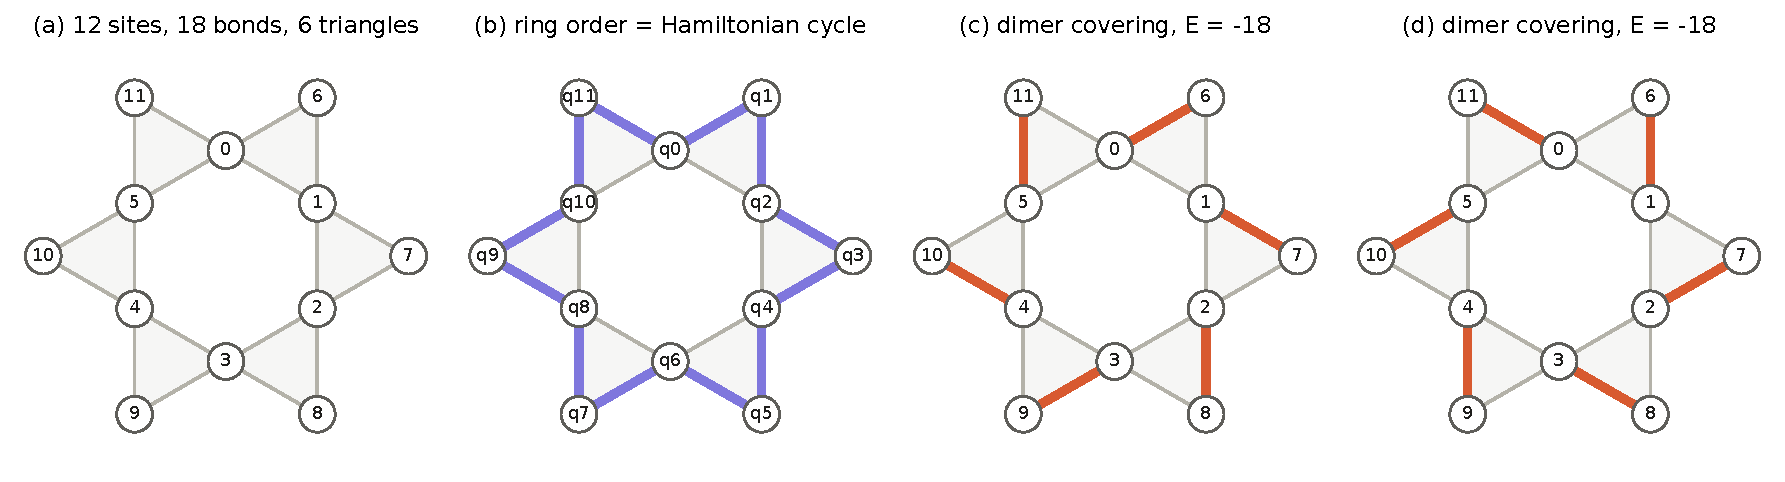
\includegraphics[width=\linewidth]{lattice}
  \caption{(a) The kagome star: hexagon sites 0--5, tips 6--11, six corner-sharing triangles
    (shaded). (b) The ring order used by the ansatzes: qubit $q_k$ hosts site
    $\sigma(k)$ of the Hamiltonian cycle, and the 12 ring bonds (purple) are all lattice bonds.
    (c, d) The two dimer coverings $M_1$ and $M_2$ of \cref{thm:ground}; each places one
    singlet in every triangle, so each has energy $-18$.}
  \label{fig:lattice}
\end{figure}

Figure~\ref{fig:lattice} shows the whole argument: panels (c) and (d) each put one dimer in every
triangle, and panel (b) is their union.

\subsection*{Exercises}

\begin{exer}\label{exer:allup}
  Compute $\bra{0^{12}}H\ket{0^{12}}$ and explain why the all-up state is an eigenstate of $H$.
\end{exer}
\begin{sol}
  On $\ket{00}$, $Z_iZ_j=+1$ and $X_iX_j$, $Y_iY_j$ map $\ket{00}$ to $\pm\ket{11}$ with opposite
  signs ($XX\ket{00}=\ket{11}$, $YY\ket{00}=-\ket{11}$), so $h_{ij}\ket{00}=\ket{00}$. Every one of
  the 18 bonds contributes $+1$: the energy is $+18$. More generally $h=2\SWAP-I$ and $\SWAP$
  fixes $\ket{0^{12}}$, so it is an eigenstate (the maximal-$S^z$ member of the ferromagnetic
  multiplet).
\end{sol}

\begin{exer}
  Compute $\bra{D_{M_1}}h_{ij}\ket{D_{M_1}}$ for a bond $\{i,j\}\notin M_1$, and recover
  $\bra{D_{M_1}}H\ket{D_{M_1}}=-18$ by counting bonds instead of triangles.
\end{exer}
\begin{sol}
  If $\{i,j\}\notin M_1$, sites $i$ and $j$ sit in different singlets, so the state factorises
  across them and $\langle\sigma^a_i\sigma^a_j\rangle=\langle\sigma^a_i\rangle\langle\sigma^a_j\rangle$.
  The reduced state of one half of a singlet is $I/2$, so $\langle\sigma^a\rangle=0$ and the bond
  contributes $0$. The 6 matched bonds contribute $-3$ each (\cref{lem:bond}) and the other 12
  contribute $0$: total $-18$. This counting gives the energy of $\ket{D_{M_1}}$; the triangle
  bound of \cref{thm:ground} is what proves that no state does better.
\end{sol}

\begin{prob}
  Using the loop rule of \cref{prop:overlap}, compute $|\braket{D_{M}}{D_{M'}}|$ for two
  coverings of a 12-site ring whose union consists of three loops of length 4.
\end{prob}
\begin{sol}
  Each loop contributes $2^{1-4/2}=\tfrac12$, so the overlap is $2^{-3}=\tfrac18$. Fewer, longer
  loops mean smaller overlap: $2^{L-N/2}$ with $L$ loops on $N$ sites.
\end{sol}
